% Reproduction of Fig. 3.1.2 in P. G. Ciarlet, The Finite Element Method for Elliptic Problems.
\documentclass[tikz,border=2mm]{standalone}
\usepackage{amsmath,amssymb}
\usetikzlibrary{calc,arrows.meta}

% Evaluation at a point
\newcommand{\nd}[1]{\fill (#1) circle (1.6pt);}
% Evaluation of the function and its first derivatives at a point
\newcommand{\hd}[1]{\fill (#1) circle (1.6pt); \draw (#1) circle (5pt);}
% Nodes of a Lagrange rectangle: #1,#2 lower-left corner, #3 width, #4 height,
% #5 number of subdivisions per side, #6 = 1 full grid, 0 only boundary nodes
\newcommand{\rectnodes}[6]{%
    \draw (#1,#2) rectangle ++(#3,#4);
    \foreach \i in {0,...,#5} {
        \foreach \j in {0,...,#5} {
            \pgfmathtruncatemacro{\isnode}{(\i==0) || (\i==#5) || (\j==0) || (\j==#5) || (#6==1)}
            \ifnum\isnode=1 \fill ({#1+\i*#3/#5},{#2+\j*#4/#5}) circle (1.6pt); \fi
        }
    }
}

\begin{document}
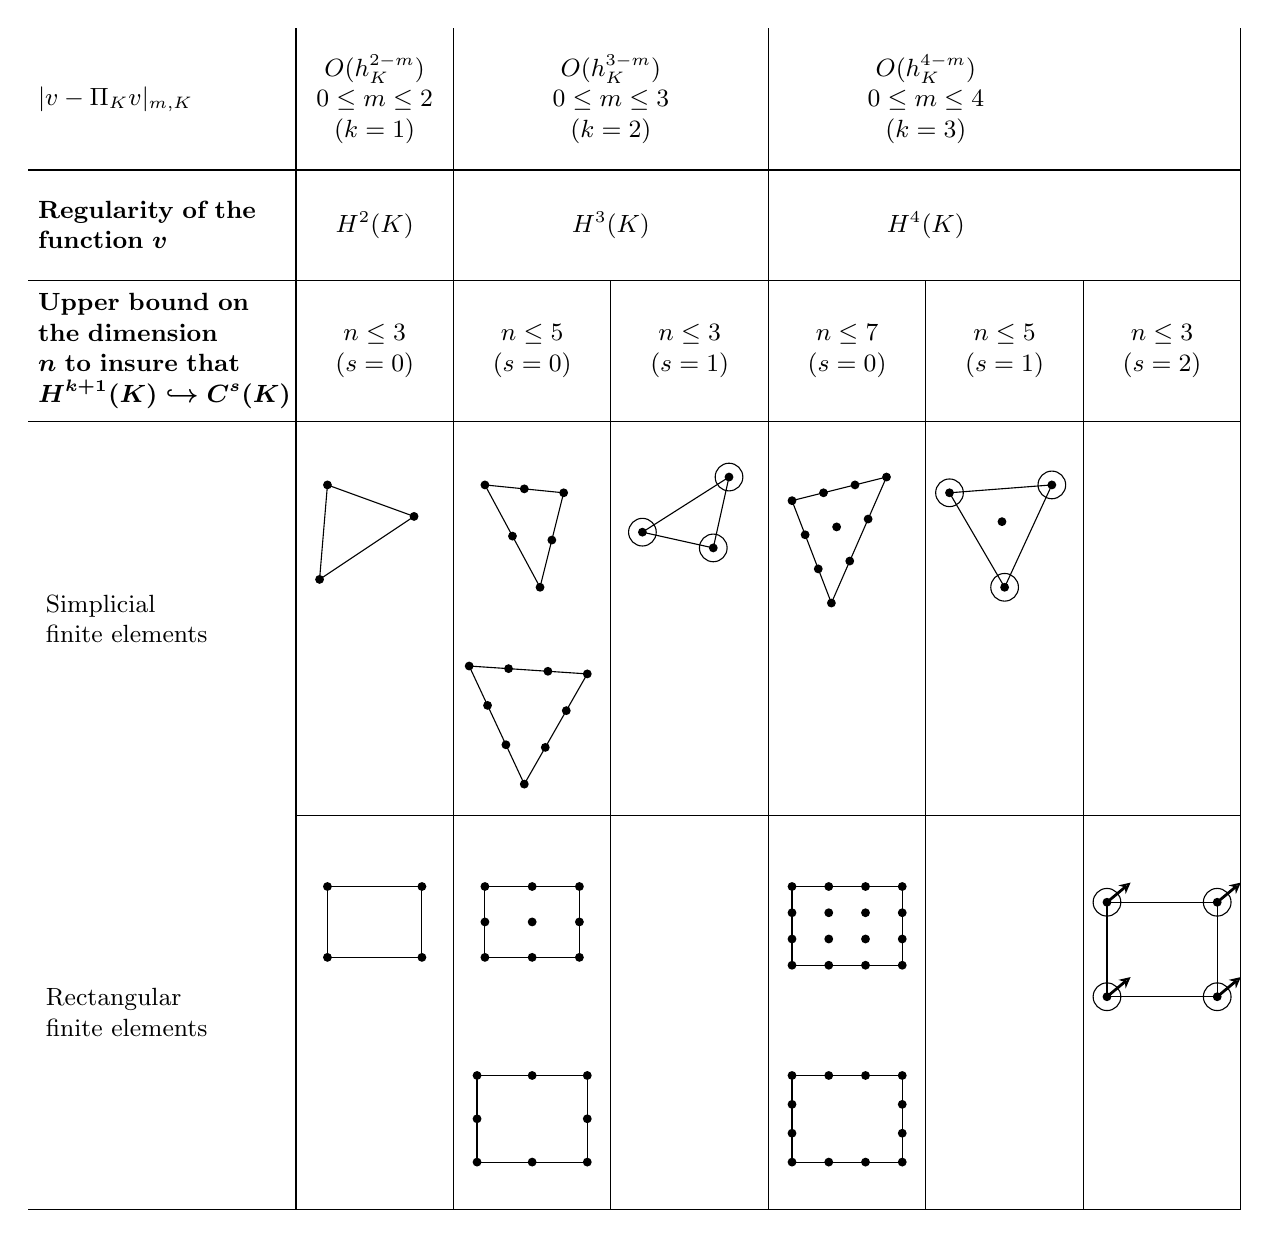
\begin{tikzpicture}[
        cell/.style={align=center, font=\small},
        label/.style={align=left, anchor=west, text width=3.5cm, font=\small},
    ]

    % Grid
    \def\L{3.4}  % end of the label column
    \def\W{2.0}  % width of each element column
    \def\R{15.4} % right border
    \foreach \y in {-1.8,-3.2,-5.0,-15.0} \draw (0,\y) -- (\R,\y);
    \draw (\L,-10.0) -- (\R,-10.0);
    \foreach \x in {\L,5.4,9.4,\R} \draw (\x,0) -- (\x,-15.0);
    \foreach \x in {7.4,11.4,13.4} \draw (\x,-3.2) -- (\x,-15.0);

    % Row 1: interpolation error
    \node[label] at (0,-0.9) {$|v - \Pi_K v|_{m,K}$};
    \node[cell] at (4.4,-0.9) {$O(h_K^{2-m})$ \\ $0 \le m \le 2$ \\ $(k = 1)$};
    \node[cell] at (7.4,-0.9) {$O(h_K^{3-m})$ \\ $0 \le m \le 3$ \\ $(k = 2)$};
    \node[cell] at (11.4,-0.9) {$O(h_K^{4-m})$ \\ $0 \le m \le 4$ \\ $(k = 3)$};

    % Row 2: regularity
    \node[label] at (0,-2.5) {\textbf{Regularity of the function $\boldsymbol v$}};
    \node[cell] at (4.4,-2.5) {$H^2(K)$};
    \node[cell] at (7.4,-2.5) {$H^3(K)$};
    \node[cell] at (11.4,-2.5) {$H^4(K)$};

    % Row 3: dimension
    \node[label] at (0,-4.1) {\textbf{Upper bound on the dimension $\boldsymbol n$ to insure that $\boldsymbol{H^{k+1}(K) \hookrightarrow C^s(K)}$}};
    \foreach \x/\n/\s in {4.4/3/0, 6.4/5/0, 8.4/3/1, 10.4/7/0, 12.4/5/1, 14.4/3/2}
    \node[cell] at (\x,-4.1) {$n \le \n$ \\ $(s = \s)$};

    % Row 4: simplicial finite elements
    \node[label] at (0.1,-7.5) {Simplicial \\ finite elements};

    % k = 1: P1 triangle
    \begin{scope}[shift={(4.4,-6.3)}]
        \coordinate (A) at (-0.6,0.5); \coordinate (B) at (0.5,0.1); \coordinate (C) at (-0.7,-0.7);
        \draw (A) -- (B) -- (C) -- cycle;
        \foreach \P in {A,B,C} {\nd{\P}}
    \end{scope}

    % k = 2, s = 0: P2 triangle
    \begin{scope}[shift={(6.4,-6.3)}]
        \coordinate (A) at (-0.6,0.5); \coordinate (B) at (0.4,0.4); \coordinate (C) at (0.1,-0.8);
        \draw (A) -- (B) -- (C) -- cycle;
        \foreach \P/\Q in {A/B,B/C,C/A} \foreach \t in {0,0.5} {\nd{$(\P)!\t!(\Q)$}}
    \end{scope}

    % k = 2, s = 0: reduced P3 triangle
    \begin{scope}[shift={(6.4,-8.7)}]
        \coordinate (A) at (-0.8,0.6); \coordinate (B) at (0.7,0.5); \coordinate (C) at (-0.1,-0.9);
        \draw (A) -- (B) -- (C) -- cycle;
        \foreach \P/\Q in {A/B,B/C,C/A} \foreach \t in {0,1/3,2/3} {\nd{$(\P)!\t!(\Q)$}}
    \end{scope}

    % k = 2, s = 1: reduced cubic Hermite triangle
    \begin{scope}[shift={(8.4,-6.3)}]
        \coordinate (A) at (-0.6,-0.1); \coordinate (B) at (0.5,0.6); \coordinate (C) at (0.3,-0.3);
        \draw (A) -- (B) -- (C) -- cycle;
        \foreach \P in {A,B,C} {\hd{\P}}
    \end{scope}

    % k = 3, s = 0: P3 triangle
    \begin{scope}[shift={(10.4,-6.3)}]
        \coordinate (A) at (-0.7,0.3); \coordinate (B) at (0.5,0.6); \coordinate (C) at (-0.2,-1.0);
        \draw (A) -- (B) -- (C) -- cycle;
        \foreach \P/\Q in {A/B,B/C,C/A} \foreach \t in {0,1/3,2/3} {\nd{$(\P)!\t!(\Q)$}}
        \nd{$(A)!2/3!($(B)!0.5!(C)$)$}
    \end{scope}

    % k = 3, s = 1: cubic Hermite triangle
    \begin{scope}[shift={(12.4,-6.3)}]
        \coordinate (A) at (-0.7,0.4); \coordinate (B) at (0.6,0.5); \coordinate (C) at (0,-0.8);
        \draw (A) -- (B) -- (C) -- cycle;
        \foreach \P in {A,B,C} {\hd{\P}}
        \nd{$(A)!2/3!($(B)!0.5!(C)$)$}
    \end{scope}

    % Row 5: rectangular finite elements
    \node[label] at (0.1,-12.5) {Rectangular \\ finite elements};

    % k = 1: Q1 rectangle
    \rectnodes{3.8}{-11.8}{1.2}{0.9}{1}{1}
    % k = 2, s = 0: Q2 rectangle and its serendipity version
    \rectnodes{5.8}{-11.8}{1.2}{0.9}{2}{1}
    \rectnodes{5.7}{-14.4}{1.4}{1.1}{2}{0}
    % k = 3, s = 0: Q3 rectangle and its serendipity version
    \rectnodes{9.7}{-11.9}{1.4}{1.0}{3}{1}
    \rectnodes{9.7}{-14.4}{1.4}{1.1}{3}{0}

    % k = 3, s = 2: Bogner-Fox-Schmit rectangle
    \begin{scope}[shift={(14.4,-11.7)}]
        \draw (-0.7,-0.6) rectangle (0.7,0.6);
        \foreach \x/\y in {-0.7/-0.6, 0.7/-0.6, 0.7/0.6, -0.7/0.6} {
                \hd{\x,\y}
                \draw[line width=1pt, -{Stealth[open,length=4pt,width=4pt]}] (\x,\y) -- ++(0.3,0.25);
            }
    \end{scope}
\end{tikzpicture}
\end{document}
